\documentclass[12pt]{article}
\usepackage{amsmath,amsfonts,amsthm,amssymb}
\usepackage[pdftex,colorlinks=true,linkcolor=black,citecolor=black,urlcolor=blue]{hyperref}
%\newcommand{\href}[2]{}
\usepackage{graphicx}
\usepackage{fullpage}

\usepackage{amscd}
\usepackage{amsmath}
\usepackage{amssymb}
\usepackage{amsthm}
\usepackage{amsfonts}
\usepackage{xxcolor}

\newtheorem{question}{Question}
\newtheorem{proposition}{Proposition}
\newtheorem{conjecture}{Conjecture}
\newtheorem{problem}[conjecture]{Problem}
\theoremstyle{definition}
\newtheorem{definition}{Definition}

\newcommand{\dd}{{\boldsymbol{d}}}
\newcommand{\ee}{{\boldsymbol{e}}}
\newcommand{\ii}{{\boldsymbol{i}}}
\newcommand{\jj}{{\boldsymbol{j}}}
\newcommand{\DD}{\boldsymbol{D}}

\newcommand{\N}{\mathbb{N}}
\newcommand{\NZ}{\mathbb{N}_0}
\newcommand{\Z}{\mathbb{Z}}
%\newcommand{\Q}{\mathbb{Q}} %should not be used throughout
\newcommand{\QP}{\mathbb{Q}_+}
\newcommand{\R}{\mathbb{R}}
\newcommand{\C}{\mathbb{C}}
\newcommand{\RP}{\mathbb{R}_+}
\newcommand{\RI}{\R_{>1}}
\newcommand{\RII}{\R_{\ge 1}}
\newcommand{\then}{\Longrightarrow}
\newcommand{\mt}[1]{\quad\mbox{#1}\quad}
\newcommand{\wo}{\setminus}
\newcommand{\wose}{\setminus^{\negmedspace\circ}}
%\DeclareMathOperator{\discup}{\dot{\cup}}
\newcommand{\discup}{\cup}
\newcommand{\propref}[1]{proposition \ref{#1}}
\newcommand{\defref}[1]{definition \ref{#1}}
\newcommand{\ra}{r.h.\ }
\newcommand{\rae}{r.h}
\newcommand{\rh}{\varrho}
\newcommand{\eps}{\varepsilon}
\newcommand{\ph}{\varphi}

\newcommand{\tothe}{\uparrow}
\newcommand{\tetr}{\uparrow\uparrow}
\newcommand{\tet}[2]{{{}^{#2}{#1}}}
\newcommand{\tlog}[2]{\tlogs_{#1}(#2)}
\newcommand{\iter}[2]{{#1}^{\langle{#2}\rangle}}
\DeclareMathOperator{\tlogs}{tlog}
\DeclareMathOperator{\id}{id}

\begin{document}
\title{
\vskip2cm 
\bf \Huge Tetration FAQ
\vskip17pt
}
\author{
Henryk Trappman \\
Andrew Robbins
}
\date{
\vskip8pt 
\today
\vskip1cm 
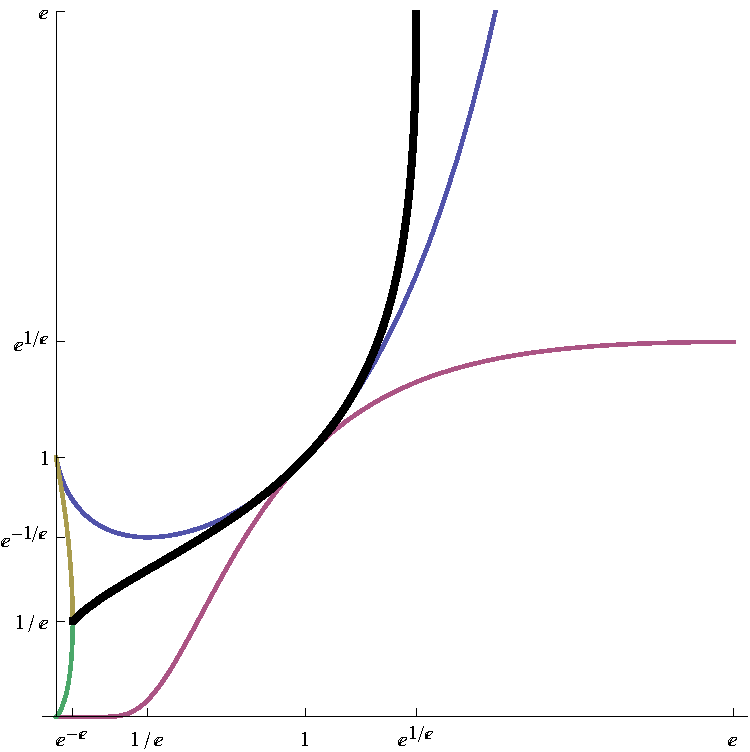
\includegraphics[width=4in]{images/plot-selfroot-plus.pdf} 
}
\maketitle
\thispagestyle{empty}
\pagebreak
\tableofcontents

\pagebreak
%\pagestyle{headings}

% ####################
% ##### Section  #####
% ####################

\section{Introduction}

This FAQ is designed to provide a basic understanding about tetration and
its related topics. This FAQ should also prevent researchers from reinventing the wheel and instead allow them to shine their light on undeveloped topics. Revealing dead-end ideas prevents authors from wasting their time and effort. It is hoped that this FAQ makes current tetration research more effective and fruitful. For questions not covered here, there is a {\bf Tetration Reference} (Ref.), available from 
\href{http://math.eretrandre.org/tetrationforum/index.php}{\tt http://math.eretrandre.org/tetrationforum/}.

\subsection{Who should read this}
This FAQ should be understandable for undergraduates (or advanced high school students) who have completed a few calculus-level math classes. Although higher math is not required, it helps. Basic knowledge of calculus, power series, and linear algebra is assumed.

\subsection{Background}
The idea of tetration enjoys great popularity among both students and lay
mathematicians. Many people have rediscovered tetration in different ways, mostly because there are many problems that tetration solves. 
When large numbers are too big, tetration is a solution. 
When the hyper operation sequence just stops, tetration is a solution. 
However, when tetration is not the solution, but the problem, then the burning central question is:
%begins with addition ($x + y$), multiplication ($xy$), exponentiation ($x^y$),

\begin{center}
\it What is the most ``beautiful'' extension of tetration beyond integers?
\end{center}

We can see immediately that this question is slightly outside the realm of
mathematics and more in the realm of taste. Perhaps this is the
reason why professional mathematicians have barely considered this
question. A more mathematical task would be to find existence and uniqueness
conditions for an extension of tetration, then find it.

What has happened is just the opposite. Dozens of authors have constructed extensions, but their uniqueness conditions remain unknown. So the initial problem of existence and uniqueness has been solved (at least 10 extensions exist), but the problem has now evolved into a search for a {\it new} problem which {\it does} admit a unique solution. Needless to say, the new problem must be ``beautiful'' as well.

This FAQ aims to briefly present some of these extensions of tetration so as to overview the methods that are available. This is partly to provide a sense of a fair competition, and partly to appeal to the taste of the reader, although we do not describe all methods here.
For a more complete description of all extensions, see Ref-4.4.
%[Note however that it will take some time until finished.]

\subsection{Acknowledgments}
We appreciate any suggestions and contributions for improving and extending it 
%(and if merely on the level of the English language which is not my native language). 
If you contribute a chapter your name will be listed here.

\subsection{Contact}
The main point of communication is the 
\href{http://math.eretrandre.org/tetrationforum/index.php}{Forum}, but if you wish to send us email:

\begin{center}
\begin{tabular}{|c|c|}
\hline
Name & Email (with obvious change) \\
\hline
Andrew Robbins & {\tt and\_j\_rob(AT)yahoo.com} \\
Henryk Trappman & {\tt bo198214(AT)eretrandre.org} \\
\hline
\end{tabular}
\end{center}

% ####################
% ##### Section  #####
% ####################

\section{Iteration}

\begin{question}
What is iteration?
\end{question}
Iteration is the process of repeating a function. Given $f(x)$ this is as simple as $f(f(x))$. The problems arise when one begins to ask questions regarding the iteration, like {\it does it converge?} or {\it can it be interpolated?}. The first question falls in the subject of dynamical systems, and the second question falls in the subject of interpolation.

Interpolation is the process of taking a list of points $(x, f(x), f(f(x)), f(f(f(x))), \ldots)$ and connecting them with a new function that that passes through each point. For example, the new function will evaluate to $F(1, x) = f(x)$, $F(2, x) = f(f(x))$ and so on. 

\begin{question}
What is iteration classified under?
\end{question}
There are two formal subject categories in the American Mathematical Society's (AMS) Mathematics Subject Classification system (at \href{http://www.ams.org/msc/}{\tt http://www.ams.org/msc/}) which describe iteration theory, which are {\bf dynamical systems} (37-xx) and {\bf functional equations} (39-xx). 

\begin{question}
How is iteration written?
\end{question}
Iteration is written $f^n(x)$, although here we use the notation $\iter{f}n(x) = f(\iter{f}{n-1}(x))$ where $\iter{f}1(x) = f(x)$ for clarity. In ASCII, iteration can be written {\tt f{\textasciicircum}n(x)} or {\tt f<n>(x)}.

\begin{question}
What terms are used with iteration?
\end{question}
In general the expression $\iter{f}n(x)$ is just referred to as {\bf iteration}, but if either $n$ or $x$ is constant, then we use slightly different names. When $n$ is constant, we call the function $x \mapsto \iter{f}n(x)$ the $n$-th {\bf iterate} of $f(x)$. When $x$ is constant, we call the function $n \mapsto \iter{f}n(x)$ the {\bf iterational} from $x$ of $f(x)$.

\subsection{Iteration of functions}
\begin{question}
It is possible to iterate a function non-integer times?
\end{question}
Short answer: it depends. 

Given a differentiable function with a formal power series, and its power series can be used as a means to study its iterates and interpolate between them, and in some cases, this interpolation also produces an differentiable function as well.

Given a function which is not continuous or differentiable, it is possible to interpolate between iterates of the function, but there are many more possible ways of doing this.

\begin{question}
What is the iteration of $\ee^x - 1$?
\end{question}
The function $\ee^x - 1$ is one of the simpler applications of continuous iteration. The reason why is because regular iteration requires a fixed point in order to work, and this function has a very simple fixed point, namely zero: $\ee^0 - 1 = 0$.


\subsection{Extension of functions}

This part is a discussion about extending the domain of functions beyond their original domain. This usually means extending a function from the integers to the real numbers, although the term {\it extension} applies to any sets. We will continue the questions later.

\subsubsection{Extension of the gamma function}
Let us illustrate the problem of extending tetration with the well-known extension of the
\href{http://en.wikipedia.org/wiki/Gamma_function}{Gamma function} and
with the well-known extension of exponentiation.

 The factorial function $n\mapsto n!$ which is
defined on the natural numbers inductively by
\begin{align*}
  1!&=1 & (n+1)!&=n!(n+1)
\end{align*}
shall be extended to have also values for fractional/real arguments
between two consecutive natural numbers, of course not any values but
certain nice, smooth, fitting values (whatever that means). We seek for
conditions that that narrow the range of possible solutions. 
The first natural condition is to satisfy the recurrence relation also
for real values, i.e. an extension $f\colon\RP\to\RP$ of the factorial
function shall satisfy
\begin{align}
  f(1)&=1 & f(x+1)=(x+1)f(x)\label{factorial recurrence}
\end{align}
for all positive real numbers $x$. This particularly forces 
$f(n)=n!$ for natural numbers $n$, i.e.\ it implies $f$ being an
extension of $n\mapsto n!$. If $f(x)$ is defined on
the open interval $(0,1)$ then this condition determines the values of
$f(x)$ for $x>1$ by induction as you can easily verify. However we can
arbitrarily define $f(x)$ on $(0,1)$ and so get infinitely many
solutions that satisfy \eqref{factorial recurrence}.
The next obvious demand is continuity, differentiability or even
analyticity of $f$. However it is well-known that another criterion
suffices:
\begin{proposition}
  The condition \eqref{factorial recurrence} together with
  logarithmic convexity, i.e.\ 
  \begin{align*}
    f(\lambda x + (1-\lambda) y)\le f(x)^\lambda
    f(y)^{1-\lambda}\mt{for all}x,y>0,0<\lambda<1,
  \end{align*}
  uniquely determine $f$ to be
  $f(x)=\Gamma(x+1)$. 
\end{proposition}

\subsubsection{Extension of exponentiation}
Till now let us having defined the exponentiation for natural
exponents by
\begin{align*}
  b^1&=b & b^{n+1}&=bb^n
\end{align*}
for real $b$ and natural $n$. 
In comparison with the Gamma function we have
the additional parameter $b$. We can anyway try to repeat the
considerations for the Gamma function by fixing $b$ in the beginning,
i.e.\ to find a function $f_b$ that satisfies
\begin{align}
  f_b(1)&=b & f_b(n+1)=bf_b(n)\label{exponentiation functional recurrence}
\end{align}
Logarithmic convexity here is somewhat self referential as we need the
power for real exponents to be defined in the expression
\begin{align*}
  f_b(\lambda x + (1-\lambda)y)\le f_b(x)^\lambda f_b(y)^{1-\lambda}
\end{align*}
So it seems as if this way is not working here (if however someone
would like to explore this in a bit more depth I would be happy to
hear about the results.)

Now we can easily generalise the original recurrence by induction to
$b^{m+n}=b^mb^n$ and by repeated induction to our key relation
\begin{align}
  b^1&=b & (b^n)^m&=b^{nm}.\label{exponentiation condition}
\end{align}
This condition if demanded for real $m$ and $n$ already suffice to
uniquely extend exponentiation to fractional exponents. For example
take $b^{\frac{1}{2}}$. If it has a value at all then must
\begin{align*}
  (b^{\frac{1}{2}})^2 = b^{\frac{1}{2}2} = b^1 = b
\end{align*}
which means that $b^{\frac{1}{2}}$ is the solution of the equation
$x^2=b$. To make the solution unique we restrict the base domain of
our extended exponentiation operation to the positive real
numbers. And then we similarly get that $b^{\frac{1}{n}}$ is the
solution of $x^n=b$, i.e.\ $b^{\frac{1}{n}}=p_n^{-1}(x)$ where
$p_n(x):=x^n$ is bijective on $\RP$ and obviously
$p_n^{-1}(x)=\sqrt[n]{x}$. Also by equation
\eqref{exponentiation condition} we get then the general formula for
fractional exponents
\begin{align*}
  b^{\frac{m}{n}}=p_m(p_n^{-1}(b)).
\end{align*}
Extension to irrational arguments merely requires the function to be
continuous.
\begin{proposition}
  There is exactly one extension of the exponentiation with natural
  numbered exponents to positive real exponents
  such that the function $x\mapsto b^x$ is continuous for each $b$ and
  which satisfies 
  \begin{align}
    (b^x)^ n &= b^{xn}\label{exponentiation uniqueness}
  \end{align}
  for each $b>0$, $x\in\RP$ and $n\in\N$. 
\end{proposition}
It can be mentioned that we could replace \eqref{exponentiation
  uniqueness} by the stronger demand 
\begin{align}
  b^{x+y}=b^xb^y.\label{exponentiation additivity}
\end{align}
 Because from
this follows by induction $b^{xn}=(b^x)^n$. In that case
  we even could extend our operation to negative exponents. First we
  notice $b^{0}b^x=b^{0+x}=b^x$ and hence $b^0=1$ for $b^x\neq
  0$. Then $b^{x}b^{-x}=b^{x-x}=b^0=1$ implies $b^{-x}=1/b^{x}$.
  
  On the other hand if we need exponentiation for tetration then both
  arguments of exponentiation must be from the same domain, and the
  greatest common domain of base and exponent is $\RP$.

\subsubsection{Extension of tetration}

By the special bracketing of the tetration the equivalent of neither 
equation \eqref{exponentiation uniqueness} nor \eqref{exponentiation
  additivity} hold for all $m,n$, i.e.\ for most $m,n\in\N$ we have: 
\begin{align}
  \tet{x}{n+m} &\neq \left({}^nx\right)^{{}^m x}\\
  {}^{nm}x &\neq {}^n({}^m x)
\end{align}
Even
\begin{proposition}
  There is {\em no} operation $\ast$ on $\RP$ such that
  \begin{align*}
    \tet{x}{n+m}=\tet{x}{m}\ast\tet{x}{n}
  \end{align*}
\end{proposition}
\begin{proof}
  Suppose there is such an operation, then we gain the contradiction
  \begin{align*}
    65536=2^{2^{2^2}}=\tet{2}{4}=\tet{2}{2+2}=\tet{2}{2}\ast
    \tet{2}{2}=4\ast 4=\tet{4}{2}=4^4=256
  \end{align*}
\end{proof}
This breaks applying the procedure of extending the exponentiation to
extending the tetration. This shall be mentioned with all insistence.
Though we have seen that $t_n(x)={}^nx$ is bijective on $\RI$ for
each $n$, a definition of ${}^{\frac{1}{n}}b$ as $t_n^{-1}(b)$ is as
arbitrary as defining it to be $\frac{\pi}{3}$.

If we want to have a unique solution we need conditions that make the
solution unique. Till now there aren't known such conditions. However
there are several conditions that one certainly want to have satisfied
for an (to some real numbers) extended tetration. 

1. The recurrence relations
\eqref{tetration start} and \eqref{tetration step}
shall be satisfied for arbitrary exponents:
\begin{align}
  \tet{b}{1} &= x & \tet{b}{x+1} &= b^{\tet{b}{x}}.\label{tetration
  recurrence}
\end{align}
This particularly implies that it is an extension of the tetration for
natural exponents.

2. The function $x\mapsto \tet{x}{a}$ shall be continuous and
strictly increasing for each $a$ (so that we can define the inverse: a
tetration root). Note that this condition suggests to restrict the
base to $\RI$ (similarly the base of exponentiation is restricted to
$\RP$).

3. The functions $x\mapsto \tet{b}{x}$ shall be continuous and
strictly increasing for each $b$ (so that we can define the inverse: a
tetration logarithm).

\begin{definition}
  A tetration extension $(x,y)\mapsto \tet{x}{y}\colon I\times
  J\to\R$, where $I,J\subseteq\R$ is called a {\em real tetration} if
  it satisfies conditions 1, 2 and 3.
\end{definition}
Additional demands could be infinite differentiability or even
analyticity. 

\subsection{Extensions of iteration}
TODO

\subsubsection{Regular iteration}
%adapted from Helmss' ContinuousFunctionalIteration.pdf
To understand {\it regular iteration} one needs to understand power series, so it is best to start with the various type of power series. 


\subsubsection{Natural iteration}
TODO

\subsubsection{Abel functional equation}
Closely related to continuous iteration is the translation equation
\begin{align*}
  F(F(a,x),y)=F(a,x+y)
\end{align*}
(if we write $F(a,x) = f^{\circ x}(a)$).
\begin{proposition}
  If $f(x):= F(b,x)$ is continuous and strictly increasing for
  one $b$ and if $F$ satisfies the translation equation (for all
  arguments of its domain of definition) then 
  \begin{align}
    F(a,x)=f_c(f_c^{-1}(a)+x)\label{translation abel}
  \end{align}
  for any $c$, where $f_c(x):=f(x+c)$. Vice versa
  $G(a,x):=g(g^{-1}(a)+x)$ satisfies the translation equation 
  for each strictly increasing continuous $g$, then $x\mapsto G(a,x)$ is
  strictly increasing and continuous for every $a$.
\end{proposition}
If we now want to real iterate a function $g$, i.e.\ $g(x)=F(x,1)$ and
  $F$ satisfies the translation equation, $x\mapsto F(a,x)$ is strictly
  increasing and continuous. Then we merely need to find a strictly
  increasing continuous function $f$ (which will be equal to $F(a,x)$
  for some $a$) such that $g(x)=F(x,1)=f(f^{-1}(x)+1)$. Or if we put
  $h:=f^{-1}$ such that
  \begin{align*}
    h(g(x))=h(x)+1
  \end{align*}
  which is the so called Abel equation.

% ####################
% ##### Section  #####
% ####################

\section{Tetration}

\begin{question}
What is tetration?
\end{question}
{\bf Tetration} is an {\it iterated exponential}, a function (on $\R \times \N \rightarrow \R$) defined as
\begin{equation}
{}^{n}x := \underset{n}{\underbrace{x^{x^{\cdot^{\cdot^{x^x}}}}}}
\end{equation}
where $n$ is called the {\bf height} and $x$ is called the {\bf base}. 
%In 1947, R. L. Goodstein coined the term {\it tetration}, along with terms for higher operations: {\it pentation}, {\it hexation}, and so on, giving each right-associative hyper-operations a short name.

Multiplication is repeated addition, exponentiation is repeated
multiplication, in similarity to this process one tries to define the
next higher operation as repetition of the exponentiation. For better
readability we introduce the symbol $\uparrow$ for exponentiation,
i.e. $x\uparrow y:=x^y$. There is however a difficulty with repeating
exponentiation because the operation is not associative (as addition
and multiplication are) so we have to chose a certain bracketing
scheme. Right bracketing seems to make the most sense (see chapter
\ref{alternative bracketings} for other bracketing schemes) and so
tetration $(x,n)\mapsto \tet{x}{n}\colon \R\times\N\to \R$ is defined as
\begin{align*}
  \tet{x}{n} := \underbrace{x\tothe (x \tothe( \dotsb \tothe x)\dotsb))}_{n\times x}
\end{align*}
or more formally inductively by
\begin{align}
  \tet{x}{1} &:= x\label{tetration start}\\
  \tet{x}{n+1} &:= x^{\tet{x}{n}}\label{tetration step}.
\end{align}
$n$ is called the (tetration) exponent and $x$ is called the
(tetration) base. 

The functions $x\mapsto \tet{x}{n}$ show an interesting behaviour in
the interval $(0,1)$. It strikingly resembles the behaviour of the
polynomials $x\mapsto x^n$ in $(-\infty,0)$. Let us have a look at the
graphs.
%\begin{figure*}[htbp]
%  \centering
%  \includegraphics[scale=0.5]{tetrations}
%\end{figure*}
%In the area where $x<1$ the graphs in ascending order are:
%$\tet{x}{1}$, $\tet{x}{3}$, $\tet{x}{5}$, $\tet{x}{6}$, $\tet{x}{4}$,
%$\tet{x}{2}$ for $x>1$ the ascending order is
%$\tet{x}{1},\dotsc,\tet{x}{6}$. 
%\begin{proposition} The function $x\mapsto \tet{x}{n}$ is bijective on
%  $\RI$ for each $n\in\N$. The function $x\mapsto \tet{x}{n}$ is bijective on
%  $\RP$ if and only if $n$ is uneven and
%  \begin{align*}
%    \lim_{x\downarrow 0} \tet{x}{n} &=
%    \begin{cases}
%      0 &\text{for uneven $n$}\\
%      1 &\text{for even $n$}
%    \end{cases}
%  \end{align*}
%\end{proposition}
This gives rise to define the inverse operation.

%20070809 Trappmann's 3.3 "Extension of Tetration"
%20070809 Trappmann's 4.2 "Tetration versus Iterated Exp"


\begin{question}
How do you make the infinite tetration fractal?
\end{question}

\begin{question}
What is repeated exponentiation?
\end{question}
%20070809 Trappmann's 2 "Tetration and Ackermann Function"
Repeated addition is multiplication, repeated multiplication is exponentiation, so is the next one repeated exponentiation? No.
The difficulty is that exponentiation is not associative,
so we have to chose a bracketing scheme. Right bracketing gives {\it the} hyper-operations, left bracketing gives lower hyper-operations, balanced bracketing gives balanced hyper-operations, and mixed bracketing gives mixed hyper-operations.

\begin{question}
What is iterated exponentiation?
\end{question}

Exponentiation $({\uparrow})$ is a binary function, so there are two ways of iterating it. $({\uparrow}c)$ is a function from $x$ to $x^c$, which is called a {\bf power} function. An {\it iterated power} function gives $({\uparrow}c)^{\circ n}(x) = ((x^c)^{\cdots})^c = x^{c^n}$. For the other way, $(b{\uparrow})$ is a function from $x$ to $b^x$, which is called an {\bf exponential} function. An {\it iterated exponential} function gives $(b{\uparrow})^{\circ n}(x)$ which is not expressible in any standard closed form.

\begin{question}
What is $a$ to the $b$th power $c$ times?
\end{question}
It depends on interpretation, since this is unclear. Assuming $b$ is repeated $c$ times:
\begin{itemize}
\item If it means: $((a{\uparrow}b){\uparrow}{\cdots}{\uparrow}b){\uparrow}b = a^{b^c}$ then it is {\it iterated powers}
\item If it means: $((b{\uparrow}b){\uparrow}{\cdots}{\uparrow}b){\uparrow}a = (b^{b^{c-1}})^a$  then it is a power of {\it iterated powers}
\item If it means: $a{\uparrow}(b{\uparrow}{\cdots}{\uparrow}(b{\uparrow}b)) = a^{({}^{c}b)}$ then it is an exponential of {\it tetration}
\item If it means: $b{\uparrow}(b{\uparrow}{\cdots}{\uparrow}(b{\uparrow}a)) = \exp_b^c(a)$ then it is {\it iterated exponentials}
\end{itemize}
and as always, it is better to be more clear, since there are so many interpretations.



\begin{question}
What is infinite tetration?
\end{question}
Tetration usually arises in the study of fixed points of exponential functions. Fixed points satisfy $f(x_0) = x_0$, so fixed points of exponential functions would satisfy $\exp_b(c) = b^c = c$. Replacing $c$ in the equation $c = b^c$ gives $c = b^{b^c}$ and repeating this gives 
$c = \exp_b^{n}(c)$. To eliminate the $c$ we continue indefinitely to get $c = \exp_b^{\infty}(x)$ and if $c$ is an attracting fixed point, then it doesn't matter what $x$ is, so this can be written $c = {}^{\infty}b$. 
Taking the $c$th root of the original equation gives $c^{1/c} = b$ 
meaning {\bf infinite tetration} ${}^{\infty}x$ (also known as the {\it infinitely iterated exponential}) is the inverse function of $x^{1/x}$.  It is defined as:
\begin{equation}
{}^{\infty}x := \lim_{n\to\infty} {}^{n}x = \frac{W(-\ln(x))}{-\ln(x)}
\end{equation}
for all $e^{-e}<x<e^{1/e}$ where $W$ is Lambert's $W$ function. For more information, see the Knoebel $H$-function in the chapter on special functions. \cite{Euler:Exponentialibus} and
\cite{Knoebel:ExponentialsReiterated}, also \cite{Ash:TheLimit},
\cite{MacDonnell:SomeCriticalPoints}, \cite{Baker:ComplexIteration}.


\begin{question}
How is tetration written? Which notation shall I use?
\end{question}
We propose to write exponentiation and tetration with base $x$ and
exponent $n$ as follows.
\begin{center}\begin{tabular}{l|c|c}
  Context & Exponentiation & Tetration\\\hline
  general & $x^n$ & $\tet{x}{n}$\\\hline
  symbol & $x\tothe n$ & $x\tetr n$\\\hline
  ASCII & \verb$x^n$ & \verb$x^^n$
\end{tabular}\end{center}

The notation $\tet{x}{n}$ is probably the most compact way of writing
tetration, however we have to be careful about ambiguity as for
example in $x\tet{x}{n}$. With this notation there is also some
uncertainty about whether tetration is $\RP\times\N\to\RP$ or
$\N\times\RP\to\RP$. The convention coherent with all the other
notations is however that tetration is $\RP\times\N\to\RP$.

In some situations it can be quite useful to have an operation symbol
instead merely a way of writing, for example in the specification
$\uparrow\colon \R\times\N\to\R$ (which however can be synonymously 
replaced by $(x,n)\mapsto x^n\colon\R\times\N\to \R$) or if we map
operations on operations indicated by a decoration, for example
$\ast\mapsto \ast'$ then we can write $x\uparrow'y$, or if there are
difficulties in writing or reading repeated nested levels of
exponents.

Alternative names for tetration are hyperpower (often used in
professional mathematical context) or superpower. Also the name hyper4
operator is in use. For me hyperpower and superpower sound somewhat
unspecific as there is a whole hierarchy of operations which are ``hyper''
respective the power.

\begin{question}
What terms used with tetration?
\end{question}

\begin{question}
  What is the Ackermann function?
\end{question}
Now we can repeat the process of defining the next higher
operation. Given an operation $\ast\colon X\times X\to X$ we define
the right right-bracketing iterator operation $\ast'\colon X \times \N\to
X$ as 
\begin{align*}
  x\ast' n := \underbrace{x\ast (x \ast( \dotsb \ast x)\dotsb)}_{n\times x}
\end{align*}
Then we have $xn=x+'n$, $x^n=x+''n$ and $\tet{x}{n} = x+''' n$. Verify
however that the left left-bracketing iterator operation
$\ast^{\backprime}\colon \N\times X \to X$  
\begin{align*}
  n \ast^\backprime x:= \underbrace{(\dotsb(x\ast x)\ast \dotsb x)\ast
  x}_{n\times x}
\end{align*}
yields basically the same operations $n+^{\backprime}x=nx$,
$n+^{\backprime\backprime} x=x^n$ and
$n+^{\backprime\backprime\backprime} x=\tet{x}{n}$.
In generalisation of this method define a sequence of operations
$\diamond_n\colon\N\times\N\to\N$ inductively by
\begin{align*}
  a \diamond_1 b &= a+b\\
  a \diamond_{n+1} b &= a \diamond_{n}' b 
\end{align*}
Particularly $m\diamond_2 n=mn$, $m\diamond_3 n=m^n$, $m\diamond_4
n=\tet{m}{n}$.  A similar construction was used by Ackermann 1927 in
\cite{Ackermann:ReelleZahlen}. He recursively defined a function
$\ph\colon\N\times\N\times\N\to\N$ which relates to our construction
by $\ph(a,b,n-1)= a \diamond_{n} b$ and used it to show that there are
recursive but not primitive recursive functions. A function similar to
$\ph$ is called original Ackermann function, ``original'' because
later R\'ozsa P\'eter  
introduced a simpler function which served the same
purpose and which is also usually called Ackermann function.

We can assume $\diamond_1$, $\diamond_2$ and $\diamond_3$ to be
extended to $\RP$. However because $\diamond_4$ (which is tetration) is merely
defined for natural numbered exponents (we generally call $x$ the basis and $y$
the exponent in the expression $x\diamond_n y$ for $n\ge 3$)
$\diamond_5$ which is the repetition of $\diamond_4$ can merely be
defined on $\N\times\N$.

So after extending tetration to real exponents one would aim to extend
all the following operations successively to real exponents.


\subsection{Tetration as an iterated exponential}
TODO
\begin{align}
  f^{\circ 1}(a)&=f(a) & f^{\circ x+y}(a)=f^{\circ x}(f^{\circ
  y}(a))\label{iteration}
\end{align}



%\subsubsection{Tetration versus iterated exponentials}
TODO\\

If we have a real iteration of the function then we can construct a real tetration from it, illustrated by
the example:
\begin{align*}
  \exp_b^{\circ 2}(x)&=b^{b^x}\\
  \exp_b^{\circ 2}(b)&=b^{b^b}=\tet{b}{3}
\end{align*}
\begin{proposition}
  For each real iteration $\exp_b^{\circ x}$ of the function $\exp_b$
  the operation defined by
  \begin{align}
    \tet{b}{a} = \exp_b^{\circ a-1}(b)\label{tet from it}
  \end{align}
  is a real tetration.
\end{proposition}
\begin{proof}
  \begin{align*}
    \tet{b}{1}&=\exp_b^{\circ 0}(b)=\id(b)=b\\
    \tet{b}{a+1}&=\exp_b^{\circ a}(b)=b^{\exp_b^{\circ
    a-1}(b)}=b^{\tet{b}{a}}
  \end{align*}
\end{proof}
Vice versa if we have defined a real tetration we can derive a
real iteration of $\exp_b$. Though we have to reach out
some more before.
Whenever we have a real tetration 
then the function $x\mapsto \tet{b}{x}$ maps $(0,\infty)$ to
$(1,\infty)$ and is injective. Hence we can define the tetration
logarithm by
\begin{align}
  \tet{b}{\tlog{b}{x}}:=x\label{tetration logarithm}
\end{align}
And this enables us then to define real iterations of
$\exp_b$ by the reasoning
\begin{align*}
  \exp_b^{\circ x}(a)&=\exp_b^{\circ x}(\tet{b}{\tlog{b}{a}})
  =\exp_b^{\circ x}(\exp_b^{\circ \tlog{b}{a}}(1))
  =\exp_b^{\circ x+ \tlog{b}{a}}(1)\\
  &=\tet{b}{x+ \tlog{b}{a}}
\end{align*}
\begin{proposition}
  For each real tetration $(x,y)\mapsto \tet{x}{y}$ the operation defined by
  \begin{align*}
    \exp_b^{\circ x}(a)&=\tet{b}{x+ \tlog{b}{a}}
  \end{align*}
  is a real iteration of $\exp_b$.
\end{proposition}
\begin{proof}
  \begin{align*}
    \exp_b^{\circ 1}(a) &= \tet{b}{1+ \tlog{b}{a}}
    = b^{\tet{b}{\tlog{b}{a}}}
    = b^a = \exp_b(a)\\
    \exp_b^{\circ x+y}(a) &= \tet{b}{x+y+ \tlog{b}{a}}
    = \tet{b}{x+ \tlog{b}{\tet{a}{y+ \tlog{b}{z}}}} 
    = \exp_b^{\circ x}(\exp_b^{\circ y}(a))
  \end{align*}
\end{proof}

These both translations (iteration to tetration and tetration to
iteration) are at least formally inverse. To see what this means 
let us generalise and simplify the notation.

Given a function $h$ with $h(1)=b$ (in
our case was $h=\exp_b$). Let $\mathfrak{A}$ be the set of all functions
$f(x)$ that are strictly increasing, continuous and that satisfy 
\begin{align*}
  f(1)&=b & f(x+1)&=f(h(x))
\end{align*}
for all $x$. Let $\mathfrak{B}$ be the set of
all operations $F(a,x)$ such that $x\mapsto F(b,x)$ is strictly
increasing and continuous, and such that
\begin{align*}
  F(a,1)&=h(a) & F(a,x+y)&=F(F(a,x),y)
\end{align*}
for all $x,y,a$.

Then we define in the sense of our previous considerations
the mappings $f\mapsto f^\uparrow\colon\mathfrak{A}\to\mathfrak{B}$
and $F\mapsto F^\downarrow\colon \mathfrak{B}\to\mathfrak{A}$ by 
\begin{align}
  f^\uparrow(a,x)&=f(f^{-1}(a)+x)\label{uparrow}\\
  F^\downarrow(x)&=F(b,x-1)\label{downarrow}.
\end{align}

We can see that they are formally inverse to each other in the
sense that $(f^{\uparrow})^\downarrow=f$ and
$(F^{\downarrow})^\uparrow=F$ for each $f\in\mathfrak{A}$ and
$F\in\mathfrak{B}$.
%%   That $\uparrow$ maps indeed into $\mathfrak{B}$ and $\downarrow$ maps indeed
%%   into $\mathfrak{A}$ is verified as in the previous propositions. To
%%   show that $\uparrow$ and $\downarrow$ are opposite bijections we
%%   simply verify 
\begin{align*}
  (F^\downarrow)^\uparrow(a,x)
  &=F^\downarrow({F^\downarrow}^{-1}(a)+x)
  =F(b,{F^\downarrow}^{-1}(a)+x-1)\\
  &=F(F(b,{F^\downarrow}^{-1}(a)-1),x)
  =F(F^\downarrow({F^\downarrow}^{-1}(a)),x)\\
  &=F(a,x)\\
  (f^\uparrow)^\downarrow(x)
  &=f^\uparrow(b,x-1)
  =f(f^{-1}(b)+x-1)=f(1+x-1)=f(x)
\end{align*}

But beware! We did not consider the domains of definitions yet. As we
can already see for natural iteration exponents, the domain
$D\subseteq \R\times \R$ of an $F$ may not be rectangular, but
be dependent on the second parameter:
\begin{align*}
  \exp_b^{\circ 0}=\id&\colon (-\infty,\infty)\leftrightarrow(-\infty,\infty)\\
  \exp_b^{\circ 1}=\exp_b&\colon (-\infty,\infty)\leftrightarrow(0,\infty)\\
  \exp_b^{\circ n}&\colon
  (-\infty,\infty)\leftrightarrow(\exp_b^{\circ n-1}(0),\infty)\\
  \exp_b^{\circ -1}=\log_b&\colon (0,\infty)\leftrightarrow (-\infty,\infty)\\
  \exp_b^{\circ -n}=\log_b^{\circ n}&\colon (\exp_b^{\circ n-1}(0),\infty)\leftrightarrow (-\infty,\infty)
\end{align*}
So for a given boundary function $d\colon \R\to\R$ define
$D_d=\{(x,t)\colon x\in(d(t),\infty),t\in\R\}$. So let $F\colon
D_d\to \R$ then $F^{\downarrow}\colon \R\to (\sup_{x\in\R}
d(x),\infty)$ because by
\eqref{uparrow} ${F^{\downarrow}}^{-1}$ must be defined on
$(d(x),\infty)$ for each $x\in\R$.

\subsection{Applications of tetration}
TODO
\subsubsection{Binary representation}
TODO
\subsubsection{Generating functions}
TODO
\subsubsection{Large numbers}
TODO

\subsection{Extensions of tetration}

\begin{question}
  What is the problem of extending tetration to non-integer heights?
\end{question}
The short answer is: uniqueness. There are no suitable conditions
found yet that favour a certain solution over others. 

\subsubsection{Ioannis Galidakis' bump method}
TODO\\
See \cite{Galidakis:Hyper4}.
\subsubsection{Robert Munafo's tower method}
TODO\\
See \cite{Munafo:Hyper4}.

\subsubsection{Jay D. Fox's linear method}

% This is a solution that satisfies $\tet{b}{1}=b$,
% $\tet{b}{x+1}=b^{\tet{b}{x}}$ and 
% infinite differentiability with respect to $x$, where $b>1$ and
% $x>-2$. By the first two conditions $\tet{b}{x}$ merely need to be defined on
% one of the intervals $(-\infty,-2]$, $(-2,-1]$, $(-1,0]$, $(0,1]$,
% $(1,b]$, etc.\ and is then already defined on $\R$ by the inductive reduction:
% \begin{align*}
%   \tet{b}{x} &= \log_b(\tet{b}{x+1})&\mt{for} x&\le -1\\
%   \tet{b}{x} &= b^{\tet{b}{x-1}}&\mt{for}x&> 0
% \end{align*}
% Before continuing let us ponder about negative tetration exponents. If
% we start at the interval $(1,b]$
% by $b=\tet{b}{1}=b^{\tet{b}{0}}$ we conclude $\tet{b}{0}=1$ and by
% $1=\tet{b}{0}=b^\tet{b}{-1}$ we conclude $\tet{b}{-1}=0$ and by
% $0=b^\tet{b}{-2}$ we conclude $\tet{b}{-2}=-\infty$. For $x=-1\dotsc
% 0$ there $\tet{b}{x}$ shall assume values between $0\dotsc 1$. By the
% reduction $\tet{b}{x}=$

% For easier computations ahead we will work with the inversion of
% $\tet{b}{x}$, the tetration logarithm defined by
% \begin{align*}
%   \tlog{b}{\tet{b}{x}}=\tet{b}{\tlog{b}{x}}=x
% \end{align*}
% Initially $\tlog{b}{x}$ is defined only for $x=\tet{b}{n}$ and we want
% to fill the gaps.
% If we choose a smooth (infinitely differentiable) $\tet{b}{x}$ on
% $(-1,0)$ we merely need to make the joins at $\tet{b}{k}$ for
% $k\in\N_0$ and $k=-1$ smooth too. However if one join (choose $0$) is
% smooth so are all joins. We have to guaranty that 

% The approach is to
% develop the inverse of $\tet{b}{x}$ on $(-1,0]$ into a powerseries at $0$ and chose the
% coefficients in such a way, that it is smooth at $0$ 


% Let $\tlog{b}{x}$ be developed at $0$ by the power series 
% \begin{align*}
% \tlog{b}{x}=\sum_{i=0}^\infty \frac{\nu_i}{i!} x^i
% \end{align*}
% We have to assure that 
% \begin{align*}
% \lim_{x\downarrow 0} D^k_x \tlog{b}{x}=\lim_{x\uparrow 0} D^k_x(\tlog{b}{b^x}-1)
% \end{align*}
% \begin{align*}
%   D^k_x \tlog{b}{x}|_{x=0} &= \nu_k\\
%   D_x b^{ix} &= D_x e^{xi\log(b)} = b^{ix} i\log(b)\\
%   D^k_x \tlog{b}{b^x} &= \sum_{i=0}^\infty \frac{\nu_i}{i!} D^k_x
%   b^{ix} = \sum_{i=0}^\infty \frac{\nu_i (i\log(b))^k }{i!} b^{ix} =
%   \log(b)^k \sum_{i=0}^\infty \frac{\nu_i i^k }{i!} b^{ix}\\
%   D^k_x \tlog{b}{b^x}|_{x=0}&= \log(b)^k \sum_{i=0}^\infty \frac{\nu_i i^k }{i!}
% \end{align*}
% So the $\nu_i$ must satisfy the following conditions
% \begin{align*}
%   \nu_0 &= \log(b)^0\sum_{i=0}^\infty \nu_i \frac{i^0}{i!} -
%   1=\tlog{b}{1}-1=-1\\
%   \nu_k &= \log(b)^k\sum_{i=0}^\infty \nu_i \frac{i^k}{i!}, k\ge 1.
% \end{align*}

% There is an elegant way to obtain {\em one} solution. We
% approximate a solution for $n\to\infty$ by assuming $\nu_i^{(n)}=0$ for
% $i>n$. This yields a linear equation system with $n$ variables
% $\nu_1^{(n)},\dotsc,\nu_n^{(n)}$ and $n$ equations. 

% Interestingly $\sum_{i=0}^\infty \frac{i^k}{i!}=eB_k$ where $B_k$ is
% the $k$-th Bell number and $e$ the Euler constant. But this implies
% that we can approximate alternative (different) solutions in
% dependence of a real parameter $\alpha$ by assuming
% $\nu_i(n,\alpha)=\alpha$ for $i>n$, then for $k\ge 1$ we have the
% alternative equation system
% \begin{align*}
%   \nu_k(n,\alpha) &= \sum_{i=0}^n \nu_i(n,\alpha) \frac{i^k}{i!} +
%   r_k(n,\alpha)
% \end{align*}
% where $r_k(n,\alpha)$ are real values determined by
% \begin{align*}
%   r_k(n,\alpha)&=\sum_{i=n+1}^\infty \alpha \frac{i^k}{i!} = \alpha
%   \left(eB_k-\sum_{i=0}^n \frac{i^k}{i!}\right)
% \end{align*}

% Numerical evidence
% supports that $\nu_i:=\lim_{n\to\infty} \nu_i^{(n)}$ exists for each
% $i$, that it is a solution of the infinite equation system and that
% the sum $\sum_{i=0}^\infty \frac{\nu_i}{i!} x^i$ converges in
% $[0,1)$. Actually is also unclear whether the thus defined
% $\tlog{b}{x}$ is analytic.

\subsubsection{Gottfried Helms's solution}
TODO\\
\href{http://groups.google.com/group/sci.math.research/browse_frm/thread/ea22b51bfa76c8a9/744173f195b78e1a#744173f195b78e1a}{Posting in sci.math.research}

% ####################
% ##### Section  #####
% ####################

\section{Related problems}
\subsection{Alternative definitions of exponentiation}
Making the Exponentiation Associative and Commutative
\begin{align*}
  x\bigtriangleup_1 y &= x+y\\
  x\bigtriangleup_{n+1} y &= \exp (\log(x)\bigtriangleup_n \log(y))
\end{align*}

\subsection{Alternative bracketing of exponentiation}
\label{alternative bracketings}
\subsubsection{Left Bracketing}
TODO
\begin{align*}
  \underbrace{((x^x)^{\dotsb})^x}_{n\times x} = x^{x^{n-1}}
\end{align*}
Uniqueness of the solution $(x,y)\mapsto x^{x^{y-1}}$?
\subsubsection{Balanced Bracketing}
TODO\\
$\tet{x}{1}=x$, $\tet{x}{2}=x^x$,
$\tet{x}{4}=\left(x^x\right)^{\left(x^x\right)}$,
et cetera. Generally we define {\em balanced tetration} as
\begin{align*}
  \tet{x}{2^0}&=x\\
  \tet{x}{2^{n+1}} &=
  \left(\tet{x}{2^n}\right)^{\left(\tet{x}{2^n}\right)}
\end{align*}
This reduces extending tetration to extending the iteration of
$F(x):=x^x$ because $\tet{x}{2^n}=F^{\circ n}(x)$. So if we found a
continuous iteration of $F$ then we have also found a continuous
iteration of the balanced tetration by
\begin{align*}
  \tet{x}{y}=F^{\circ \log_2(y)}(x)
\end{align*}
We can simplify the treatment of $F(x)$ by introducing $G(x):=xe^x$
(which is the inverse of the Lambert's $W$ function) and noticing that
$F^{\circ n}=exp\circ G^{\circ n} \circ \ln$ because $F:=\exp\circ
G\circ \ln$. So continuous iteration is reduced to continuous
iteration of $G$. Now $G$ has a fixed point at $0$ (corresponding to
the fixed point of $F$ at $1$) and can be developed at $0$ into the
powerseries
\begin{align*}
  G(x)=\sum_{j=1}^\infty j \frac{x^{j}}{j!}
\end{align*}
Formal powerseries of the form $x+\dotsc$ have a unique continuous
iterate. So if it converges (which seems quite so) then $G$ has a unique
continuous iterate and then $F$ has a unique continuous iterate and
then there is a unique analytic balanced tetration.

\subsection{Choose a number system that reflects non-associativity}
TODO\\
\href{http://math.eretrandre.org/tree-aoc/pdf/latest.pdf}{Arborescent
  Numbers and Higher Arithmetic Operations (article)}\\
\href{http://math.eretrandre.org/cgi-bin/ftc/ftc.pl}{Tree fraction
  calculator (web application)}



















\nocite{Wolfram:NKSOpenProblems-2003-June}

\bibliographystyle{amsplain-uhe}
\bibliography{main}

\end{document}


